Existem diversos \textit{benchmarks} que especificam e simulam cargas de trabalho para avaliarem sistemas computacionais. No entanto, não existe nenhum \textit{benchmark} que possibilite uma avaliação em regime transiente. Este capítulo apresenta e defini uma metodologia de extensão de avaliação em regime transiente para \textit{benchmarks} aproveitando toda a sua maturidade e robustez.




\section{Estratégicas de extensão}

O \textit{benchmark} bench4Q define uma carga de trabalho, incluindo banco de dados, transações, regras de execução e de taxa de transferência e métricas de resposta.  Para expor a dinâmica de um sistema é necessário estimulá-lo, a carga de trabalho é quem estimulará o sistema através de cenários ou fenômenos de \textit{burstiness}. Essa implementação é composta por classes ou funções, influenciado diretamente pela linguagem em que o \textit{benchmark} foi desenvolvido, esse conjunto de código é um componente básico do \textit{benchmark} que refere-se a uma unidade de trabalho genérico que envia a carga para o sistema. Alguns \textit{benchmarks} incluem solicitações HTTP, chamadas de procedimento remoto, invocações de serviços Web, transações de banco de dados, comandos interativos ou também mesmo poderia ser composto de múltiplas tarefas de processamento, por exemplo sessões de cliente que compreendem várias solicitações ao sistema, etc \cite{Kounev2005}. Segundo \cite{Nobile2013} uma alteração na entrada (carga de trabalho) fará com que o sistema saia do estado em regime estacionário e entre em um período de regime transiente e para descrever a dinâmica de um sistema, comumente, o ganho em regime estacionário é calculado para uma entrada degrau unitário.

O objetivo deste trabalho é estender a carga de trabalho do sistema de tal maneira que permite-se estimular o sistemas a apresentar a sua dinâmica, assim possibilitando a analise transiente do sistema.


%Comumente a avaliação de desempenho de sistemas computacionais é realizada em regime estacionário, isto é, sob carga de trabalho constante. Tradicionalmente a avaliação feita dessa forma produz dados para inferir a capacidade estática do sistema. O sistema inicialmente sem carga, é excitado com a entrada de interesse, e aguarda-se até que a saída estabilize-se no valor desejado, podendo ser um valor constante ou um valor dentro de um intervalo. A condição aceitável é alcançada passado o warm up (aquecimento), período em que o sistema encontra-se em estado de inicialização. A determinação da capacidade obtém-se estimulando o sistema com carga gradativamente mais elevadas até atingir seu limite inferior de desempenho aceitável, correspondente à carga estática máxima suportada. Análise do comportamento no período de aquecimento contém informações importantes relacionadas com a capacidade do sistema operando em condições reais onde a carga não é constante.
%Em regime transiente, a quantidade de recursos necessários para garantir o desempenho especificado pode divergir substancialmente daquela definida em regime estacionário. Durante um período transiente, as consequências duma perturbação na carga a quantidade de recursos necessários seria temporariamente superior àquela prevista para o regime de carga não variável. Isso resulta, por exemplo, em descumprimento dos níveis de serviço ou paradas no funcionamento dos sistemas.
%Dentro de um ambiente de testes local uma das principais limitações na simulação de sistemas e-commerce é o acesso ao banco de dados. Percebe-se que o banco de dados é o principal fator limitante para a analise transiente  para níveis altos de carga os dados coletados são pouco uteis, porque aparecem claros sinais de problemas de entrada e saída. 

%Devemos ter em conta que dentro da nuvem existem recursos com maior escalabilidade

%Além disso, nós quantificar a sobrecarga de desempenho para HA em comparação com o sistema de não-HA durante as operações normais. Temos utilizado este método para impulsionar melhorias na disponibilidade SQL Server. Embora a metodologia não é específico para a carga de trabalho TPC-E ou o Microsoft SQL Server, não estamos tentando definir um "uso geral" HA referência neste documento.

Para a discussão deste trabalho, assumimos um sistema consiste nos principais componentes:

\begin{description}
	\item[Servidor Físico:]
	\item[Balanceador de carga:]
	\item[Servidores Virtuais:]
	\item[Servidor de dados:]	
\end{description}

%Dependendo do grau de disponibilidade e necessidade da aplicação, um sistema de banco de dados HA pode precisar de redundância em várias camadas, como fonte de alimentação, armazenamento (por exemplo, níveis de disco RAID), NICs e switches de rede, número de instâncias de banco de dados standby, eo sistema duplicado em dados remoto central (para a recuperação de desastres geográfica). Neste artigo vamos nos concentrar em como o RDBMS lida com várias falhas. 

A carga de trabalho TPC-E é alargada para abranger os seguintes cenários de inatividade:
\begin{itemize}
	\item %• o tempo de inatividade planejado: Um período de tempo de paradas programadas para manutenção do sistema, caracterizado por uma transição ordenada de serviço de Principal para Standby Server. As causas das interrupções programadas incluem patches de OS & SQL, service pack, manutenção de hardware, manutenção on-line, etc.
	\item %• o tempo de inatividade não planejado: Um período de tempo de inatividade não programado, muitas vezes devido a vários falhas, tais como falhas de hardware, erros de software e erros humanos, causando uma transição abrupta do serviço de Principal de espera do servidor.		
\end{itemize}

Failover se refere à transição do serviço de Principal para Standby Server. Idealmente, o sistema de banco de dados pode failover automaticamente, sem intervenção administrativa para o tempo de inatividade não planejado. O administrador normalmente inicia um processo de failover 'manual' para o tempo de inatividade planejado. Failback refere-se à transferência de serviço de volta para o servidor principal original (após planejado / tempo de inatividade não planejado). A operação é muitas vezes semelhante ao failover manual, exceto que os servidores do Principal / Standby são viradas.

A Figura 1 mostra os principais componentes no ambiente de teste. Note que a definição System- Sub-Test (SUT) no benchmark TPC-E é estendido para incluir o componente de conectividade, que pode ser executado em ambos fisicamente a máquina Motorista TPC-E (por exemplo, SQL Server Native Client para Database Mirroring) ou uma máquina de servidor (por exemplo, nome de rede virtual para Failover Clustering).
Para simular o tempo de inatividade planejado, podemos chamar APIs de failover fornecidos pelo RDBMS durante a execução da carga de trabalho TPC-E. Para o tempo de inatividade não planejada, precisamos simular vários eventos perturbadores que possam ocorrer no sistema. A Tabela 1 mostra alguns exemplos de falha.

Em nosso modelo, assumimos que o sistema segue o princípio de "fail-fast 'descrito por Gray e Siewiorek [4]. Desde que as falhas em hardware e software causar falhas imediatas, não é necessário testar através de um conjunto exaustivo de modos de falha.
Assim nós não tentar enumerar uma lista "completa" de falhas. O atributo fail-fast devem ser verificadas independentemente do teste de desempenho.

3.2 Métricas
As métricas de disponibilidade precisam refletir cenários de clientes eo custo de um sistema de HA, que inclui três aspectos principais:
• O custo de capital: O custo de hardware e software adicional necessário para um sistema de HA em comparação com um sistema não-HA outra forma equivalente.
• impacto Performance: O impacto para o desempenho de recursos de alta disponibilidade durante as operações normais em comparação com o sistema de não-HA.
• Tempo de recuperação: O tempo para restaurar o serviço de banco de dados após a ocorrência de uma falha.

Caracterizando custo de capital está além do escopo deste artigo, mas acreditamos que o modelo de precificação definidos na especificação TPC-E pode ser usado como é calcular preços do sistema tanto para HA e configurações não-HA.
Para entender o impacto no desempenho durante a operação normal, vamos medir o throughput TPCE em estado estacionário em um sistema HA e comparar isso contra um sistema autônomo para caracterizar a diferença.
A definição de time-to-recover pode incluir (1) o servidor é para cima, (2) todos os dados é acessível, e (3) o sistema está de volta ao estado estacionário, ou seja, ele pode entregar uma determinada percentagem do pico throughput dentro da restrição de tempo de resposta. Neste papel a definição de tempos a recuperar é (3), que pode ser dividido em duas fases:
• o tempo de inatividade de serviço: Após uma falha ocorre, quanto tempo leva para que o sistema voltar e estar pronto para processar novas solicitações.
• Time-to-steady-estado: Como rapidamente as rampas do sistema para entregar o rendimento de estado estacionário.

A Figura 2 é um gráfico que ilustra o rendimento conceitual nossas métricas, incluindo o impacto de transferência, o tempo de inatividade do serviço e tempo de colocação no estado estacionário.

--------------------------------------------------------------------
\label{sec-method}

Diversos autores \cite{Hinnant1988, Price1989, KaiSachs2010, Folkerts2013, Marco2012} reconhecem a falta de uma metodologia estabelecida para o desenvolvimento de \textit{benchmarks}. Essa seção, apresenta uma metodologia de extensão para analise transiente através de um \textit{benchmark}. 

A metodologia de extensão descreve as etapas necessárias para as modificações, a seguinte metodologia permite que se obtenha uma carga de trabalho que estimule o sistemas a apresentar a sua dinâmica, assim possibilita a analise transiente do sistema. De acordo com \cite{KaiSachs2010}, uma metodologia de desenvolvimento de \textit{benchmarks} deve incluir o seu processo de desenvolvimento, bem como a sua execução e análise dos seus resultados. 

O objetivo da metodologia é possibilitar que qualquer \textit{benchmark} possa avaliar um sistema em regime transiente afim de descreve a capacidade de resposta e eficiência em reagir às mudanças nas condições de tempo de execução através de modificações feitas no \textit{benchmark}, não tendo a necessidade de desenvolver um; para tanto é fundamental seguir as características presente no \textit{benchmarks}, conforme descrito nessa seção.

De um modo geral, a metodologia de extensão para analise em regime transiente pode ser dividida em três fases:

\begin{enumerate}
	\item Para expor a dinâmica de um sistema é necessário estimulá-lo, a carga de trabalho é quem estimulará o sistema. Logo, a primeira fase é a identificação da implementação do gerador de carga no \textit{benchmark}. Muitas vezes, essa fase é específico para um conjunto de classes, que permite a caracterização da carga de trabalho. 
	Essa implementação é composta por classes ou funções, influenciado diretamente pela linguagem em que o \textit{benchmark} foi desenvolvido, esse conjunto de código é um componente básico do \textit{benchmark} que refere-se a uma unidade de trabalho genérico que envia a carga para o sistema. Alguns \textit{benchmarks} incluem solicitações HTTP, chamadas de procedimento remoto, invocações de serviços Web, transações de banco de dados, comandos interativos ou também mesmo poderia ser composto de múltiplas tarefas de processamento, por exemplo sessões de cliente que compreendem várias solicitações ao sistema, etc.\cite{Kounev2005}
	A escolha dos componentes de carga são definidos em função da natureza dos serviços prestados pelo sistema e sobre os objetivos de modelagem. Uma vez que, em quase todos os casos, esses componentes pode ser considerado como uma espécie de pedidos ou transações processadas pelo sistema, que, muitas vezes, se referem a eles como os pedidos e transações.\cite{Kounev2005}
		
	\begin{figure}[htb]
		\caption{Comportamento de métrica transiente}
		\label{fig:funcoes1}
		\centering
		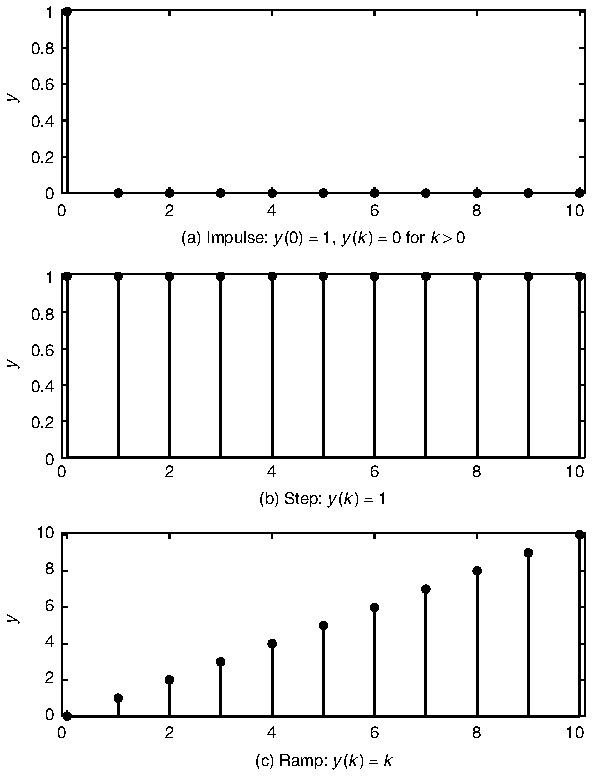
\includegraphics[scale=1]{funcoes1.pdf}
		\fdireta{Hellerstein2004}
	\end{figure}
	
	%\begin{figure}
	%	\begin{center}
	%		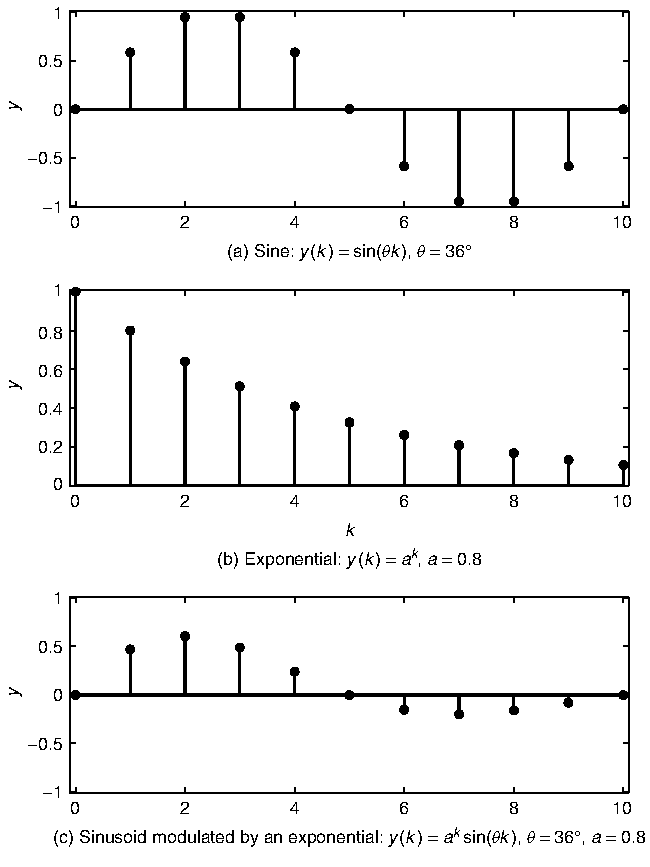
\includegraphics[width=0.8\textwidth]{img/funcoes2.pdf}
	%		\caption{Sinais em tempo discreto comuns, parte 2. \cite{Hellerstein2004}}
	%		\label{fig:funcoes2}
	%	\end{center}
	%\end{figure} 
	
	Segundo \cite{Nobile2013} uma alteração na entrada (carga de trabalho) fará com que o sistema saia do estado em regime estacionário e entre em um período de regime transiente e para descrever a dinâmica de um sistema, comumente, o ganho em regime estacionário é calculado para uma entrada degrau unitário. \textit{Para realizar a analise transitória do sistema, é preciso utilizar cargas de trabalho que possam provocar comportamentos propícios}, onde as caraterísticas dinâmicas do sistema sejam claramente observadas, em \cite{Hellerstein2004}, são propostas algumas funções, ou sinais, de perturbação, por exemplo: impulso, degrau, rampa, seno, exponencial, seno modulada por uma exponencial, etc.  Essas funções são apresentadas na figura \ref{fig:funcoes1}.% e \ref{fig:funcoes2}.
	
	Assim as modificações devem ser feitas no \textit{engine} do gerador de carga do \textit{benchmark}, pois nele que se encontra o componente que tem o conjunto de parâmetros que caracterizam a carga de trabalho. A carga de trabalho resultante deve expressar ao menos uma das funções apresentadas.
		
	
	\item O segundo passa da metodologia, é medir o comportamento do sistema com a ajuda de métricas. A métrica é uma função que transforma resultados medidos em uma forma que seja facilmente compreendida. \cite{Folkerts2013} As métricas de referência deve permitir caracterizar e quantificar o comportamento do sistema quando enfrenta perturbações (ou seja, falhas, ataques, e variações de ambiente operacional).\cite{Marco2012} As métricas tradicionais, de analise estacionaria, não pode capturar o comportamento transitório do sistema em resposta às variações de carga implementada no primeiro passo da metodologia.
	
	No contexto de avaliação transiente, \cite{Rosu1997} afirma que a reatividade da métrica é muitas vezes mais importante do que a otimização da mesma, no mesmo trabalho, \cite{Rosu1997} apresenta a característica e comportamento de uma métrica transiente, conforme ilustrado pela figura \ref{fig:transient-metric}, que são: 
	\begin{itemize}
		\item \textbf{\textit{Reaction Time} (Tempo de reação)} - o período entre a ocorrência da variação crítica e a conclusão da promulgação realocação de correção;
		
		\item \textbf{\textit{Recovery Time} (Tempo de Recuperação)}  - o intervalo entre a conclusão promulgação e da restauração de um nível de desempenho aceitável;
		
		\item \textbf{\textit{Performance Laxity} (Frouxidão performance)} - a diferença entre o required v performance, e o desempenho em estado estacionário, após a redistribuição;
	\end{itemize}
	
	
	\begin{figure}[htb]
		\caption{Comportamento de métrica transiente}
		\label{fig:transient-metric}
		\centering
		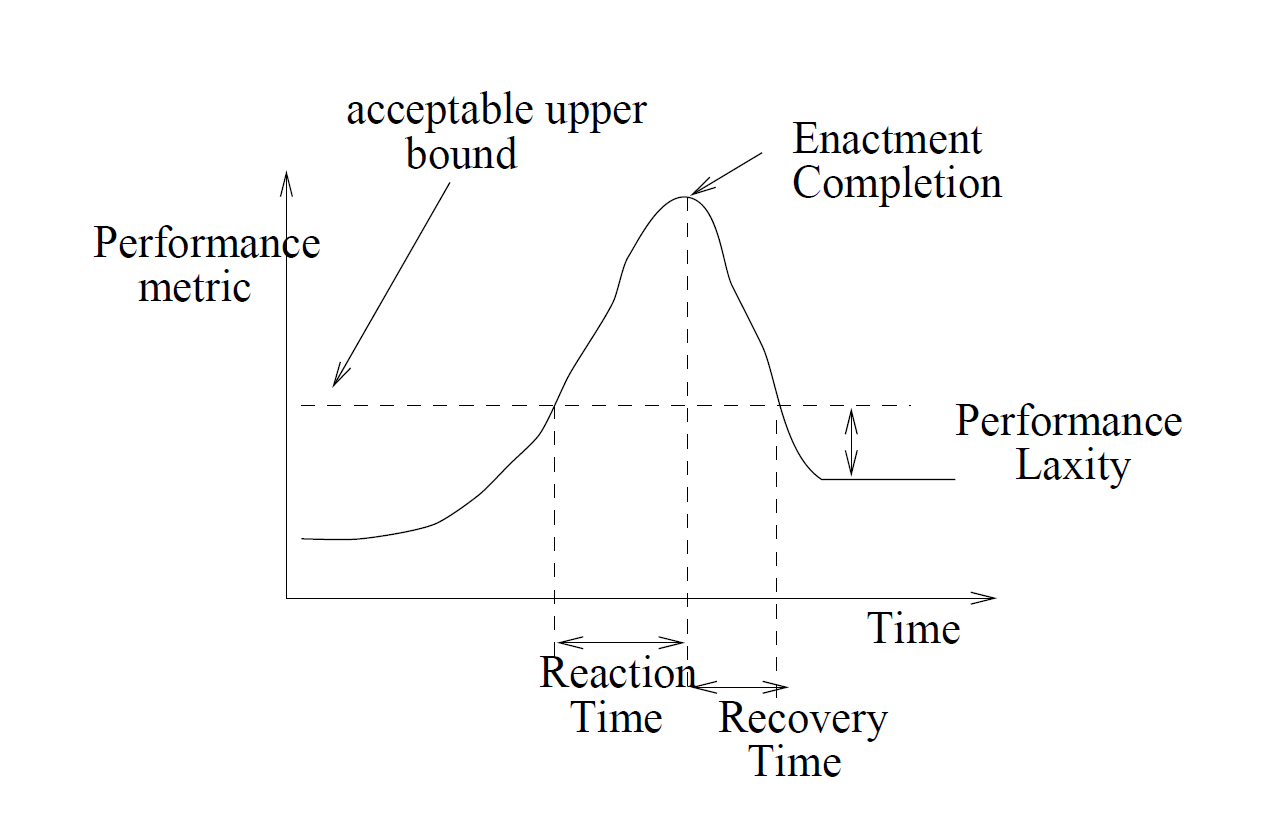
\includegraphics[scale=0.4]{transient-metric.png}
		\fdireta{Rosu1997}		
	\end{figure}
	
	
	A métrica em questão deve ser identifica dentro da realidade e necessidade em que se encontra o sistemas a ser avaliado. Logo será de uma ingenuidade fixar uma métrica para um sistema desconhecido, o importante é que ela tenha o comportamento e as caracteriais apresentadas anteriormente nesse passo da metodologia de extensão. Existem diversos trabalhos dedicados que identificam métricas transiente em vários contextos como o \cite{Binnig2009, Lu2000, Rosu1997}.
	
	\item A última atividade dentro da metodologia de extensão do \textit{benchmark} é a análise e apresentação de resultados. Aqui, os dados bruto de desempenho são obtidos estatisticamente processadas e interpretadas. Para a análise, a metodologia deve fornecer orientações para uma avaliação estatística rigorosa e validação dos dados coletados. Além disso, ele deve fornecer orientações para a apresentação dos resultados estatísticos, os intervalos de confiança presentes em adição à média. Para garantir a replicabilidade, deve, adicionalmente, fornecer diretrizes para a descrição das experiências de \textit{benchmark} realizados.		
	
\end{enumerate}




